\section{Print-out some code}

\begin{lstlisting}[caption=My Javascript Example]
/**
 * Paquito network simulation
 * 
 * @version 0.1
 */
var PKT = function () {
	var _frame = FRM;
	var _sender = SDR;
	var _reciever = RCR;
	
	var _settings = {
		debug: true, // output debug info
		debugMode: 'console', // debug output method ('console' or 'alert')
	};
	
	/**
	 * Output Paquito debug information
	 * @param {String} msg Message to print
	 */
	var _debug = function(msg) {
		msg = 'Paquito: ' + msg;
		if(_settings.debug)
		{
			switch(_settings.debugMode) {
				case 'alert':
					alert(msg);
					break;
				case 'console':
					console.log(msg);
					break;
				default:
					alert(msg);
					break;
			}
		}
	};

	var _test = function () {
		_frame.payload('01010101');
		_debug(_frame.crc());
	};
	
	/**
	 * Initialize Paquito
	 * @param {Object} settings
	 */
	var _init = function(settings) {
		for(attr in settings) {
			_settings[attr] = settings[attr];
		}
		
		_debug('Initialized');
		
		_test();
	};
	
	// expose public properties and methods
	return {
		init: _init,
	};
}();
\end{lstlisting}

\subsection{Inserting an image}

\begin{center}
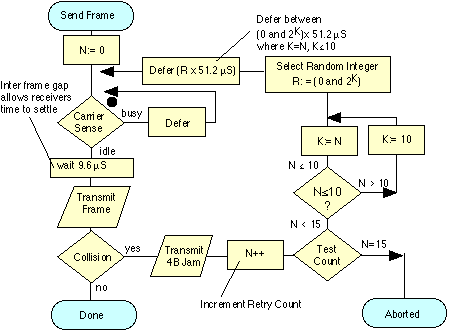
\includegraphics[scale=0.8]{ether.png}
\end{center}

